% Tento soubor nahraďte vlastním souborem s přílohami (nadpisy níže jsou pouze pro příklad)

% Umístění obsahu paměťového média do příloh je vhodné konzultovat s vedoucím
%\chapter{Obsah přiloženého paměťového média}

%\chapter{Manuál}

%\chapter{Konfigurační soubor}

%\chapter{RelaxNG Schéma konfiguračního souboru}

%\chapter{Plakát}

\chapter{Typy ASDU}
 
\begin{table}[H]
\centering
    % \begin{tabular}{|l|l|l|}
    \begin{tabularx}{\textwidth}{|c|X|l|}
        \hline
        \textbf{Code}             & \textbf{Description}                                     & \textbf{Valid COTs} \\ \hline
        \textbf{31}  & Double point information with time tag                   & 3,5,11,12           \\ \hline
        \textbf{36}  & Measured value, short floating point value with time tag & 2,3,5,11,12,20,20+G \\ \hline
        \textbf{45}  & Single command                                           & 6,7,8,9,10,44,45,46,47 \\ \hline
        \textbf{46}  & Double command                                           & 6,7,8,9,10,44,45,46,47 \\ \hline
        \textbf{100}  & (General-) Interrogation command                                            & 6,7,8,9,10,44,45,46,47 \\ \hline
        \textbf{120} & File ready                                               & 13                  \\ \hline
        \textbf{121} & Section ready                                            & 13                  \\ \hline
        \textbf{122} & Call directory, select file, call file, call section     & 5,13                \\ \hline
        \textbf{123} & Last section, last segment                               & 13                  \\ \hline
        \textbf{124} & Ack file, Ack section                                    & 13                  \\ \hline
        \textbf{125} & Segment                                                  & 13                  \\ \hline
    % \end{tabular}
    \end{tabularx}
    \caption{Vybrané kódy určující typ ASDU jednotky \cite{iec_104}.}
    \label{asdu_types_table}
\end{table}


\chapter{Kódy COT}
 
\begin{table}[H]
\centering
    \begin{tabularx}{\textwidth}{|c|X|l|}
        \hline
        \textbf{Code} & \textbf{Cause of Transmission} & \textbf{Abbreviation} \\ \hline
        \textbf{1}  & periodic, cyclic      & per/cyc \\ \hline
\textbf{2}  & background interrogation      & back \\ \hline
\textbf{3}  & spontaneous       & spont \\ \hline
\textbf{4}  & initialized       & init \\ \hline
\textbf{5}  & interrogation or interrogated         & req \\ \hline
\textbf{6}  & activation        & act \\ \hline
\textbf{7}  & confirmation activation       & actcon \\ \hline
\textbf{8}  & deactivation      & deact \\ \hline
\textbf{9}  & confirmation deactivation         & deactcon \\ \hline
\textbf{10} & termination activation        & actterm \\ \hline
\textbf{11} & feedback, caused by distant command       & retrem \\ \hline
\textbf{12} & feedback, caused by local command         & retloc \\ \hline
\textbf{13} & data transmission         & file \\ \hline
\textbf{14--19} & reserved for further compatible definitions & \\ \hline
\textbf{20} & interrogated by general interrogation         & inrogen \\ \hline
\textbf{21} & interrogated by interrogation group 1         & inro1 \\ \hline
\textbf{22} & interrogated by interrogation group 2         & inro2 \\ \hline
% \textbf{23} & interrogated by interrogation group 3         & inro3 \\ \hline
% \textbf{24} & interrogated by interrogation group 4         & inro4 \\ \hline
  & \dots & \\ \hline
\textbf{36} & interrogated by interrogation group 16        & inro16 \\ \hline
\textbf{37} & interrogated by counter general interrogation         & reqcogen \\ \hline
\textbf{38} & interrogated by interrogation counter group 1         & reqco1 \\ \hline
\textbf{39} & interrogated by interrogation counter group 2         & reqco2 \\ \hline
% \textbf{40} & interrogated by interrogation counter group 3         & reqco3 \\ \hline
% \textbf{41} & interrogated by interrogation counter group 4         & reqco4 \\ \hline
  & \dots & \\ \hline
\textbf{44} & type-Identification unknown       & uknown\_type \\ \hline
\textbf{45} & cause unknown         & uknown\_cause \\ \hline
\textbf{46} & ASDU address unknown      & unknown\_asdu\_address \\ \hline
\textbf{47} & Information object address unknown & unknown\_object\_address \\ \hline
    \end{tabularx}
    \caption{Kódy COT a jejich význam \cite{iec_104}.}
    \label{cot_table}
\end{table}

\chapter{Dialog pro načtení CSV souboru}

\begin{figure}[H]
	\centering
    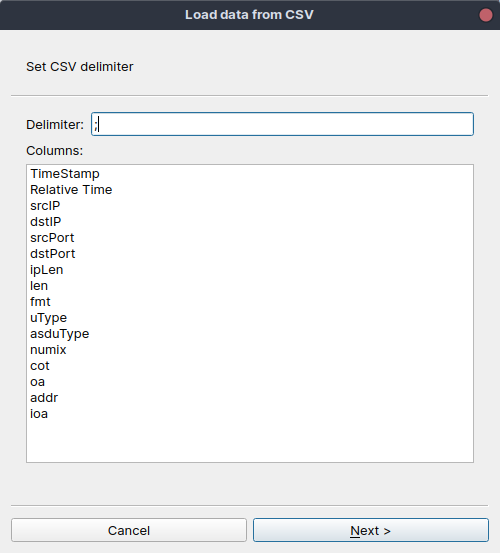
\includegraphics[width=0.5\textwidth]{obrazky-figures/load_csv_cols.png}
    \caption{Výběr oddělovače a zobrazení názvů sloupců, které by vznikly použitím zvoleného oddělovače.}
    \label{fig:delim_select_screen}
\end{figure}
    
\begin{figure}[H]
    \centering
    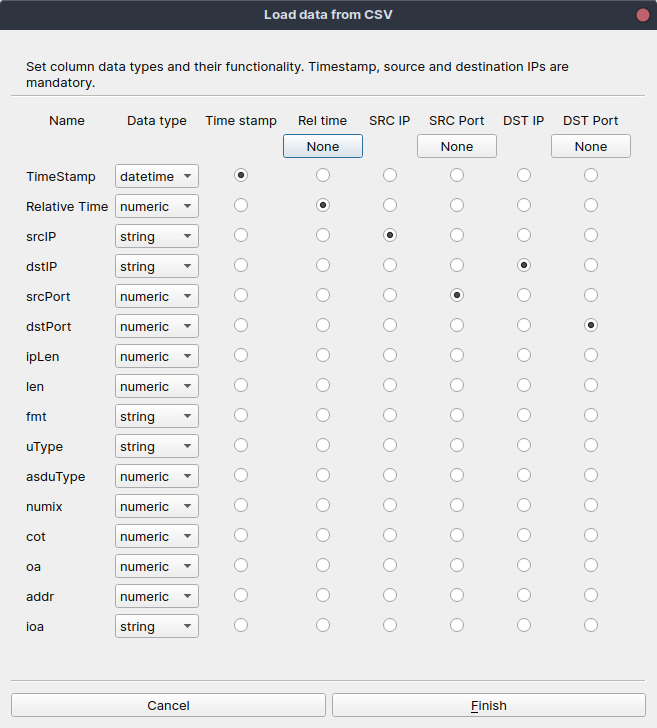
\includegraphics[width=0.75\textwidth]{obrazky-figures/load_csv_types.png}
    \caption{Výběr datových typů sloupců a sloupců reprezentujících speciální atributy.}
    \label{fig:type_select_screen}
\end{figure}


\chapter{Pohledy aplikace}
\label{panel_images}

Ukázka všech pohledů aplikace s načtenou datovou sadou D.

\begin{figure}[H]
	\centering
	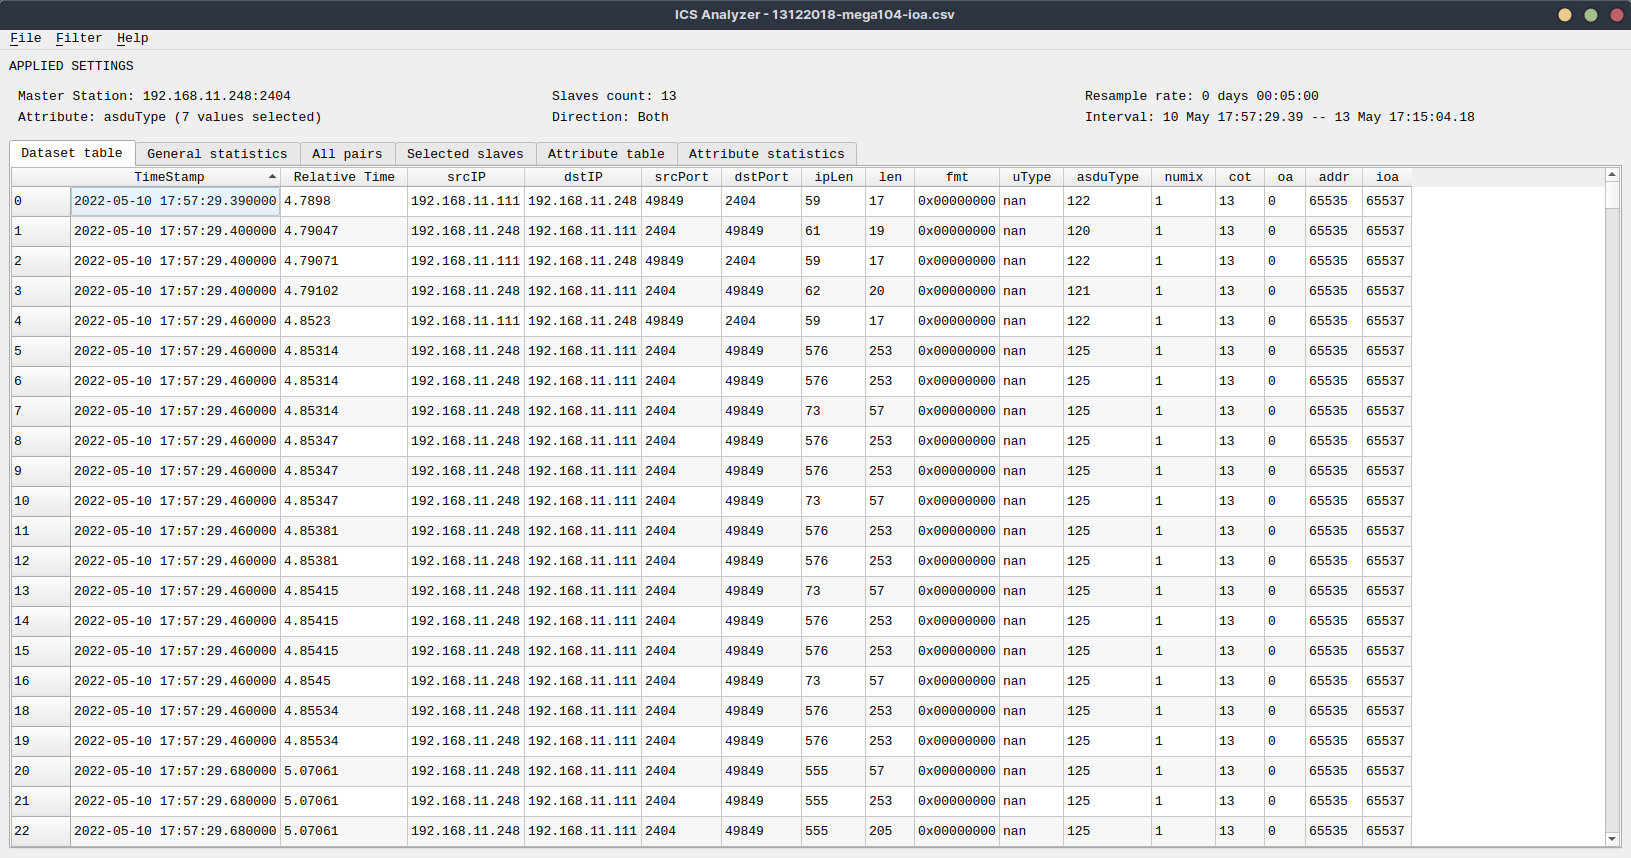
\includegraphics[width=1\textwidth]{obrazky-figures/tabs/tab1.png}
	\caption{Dataset table.}
	\label{fig:tab1}
\end{figure}



\begin{figure}[H]
	\centering
	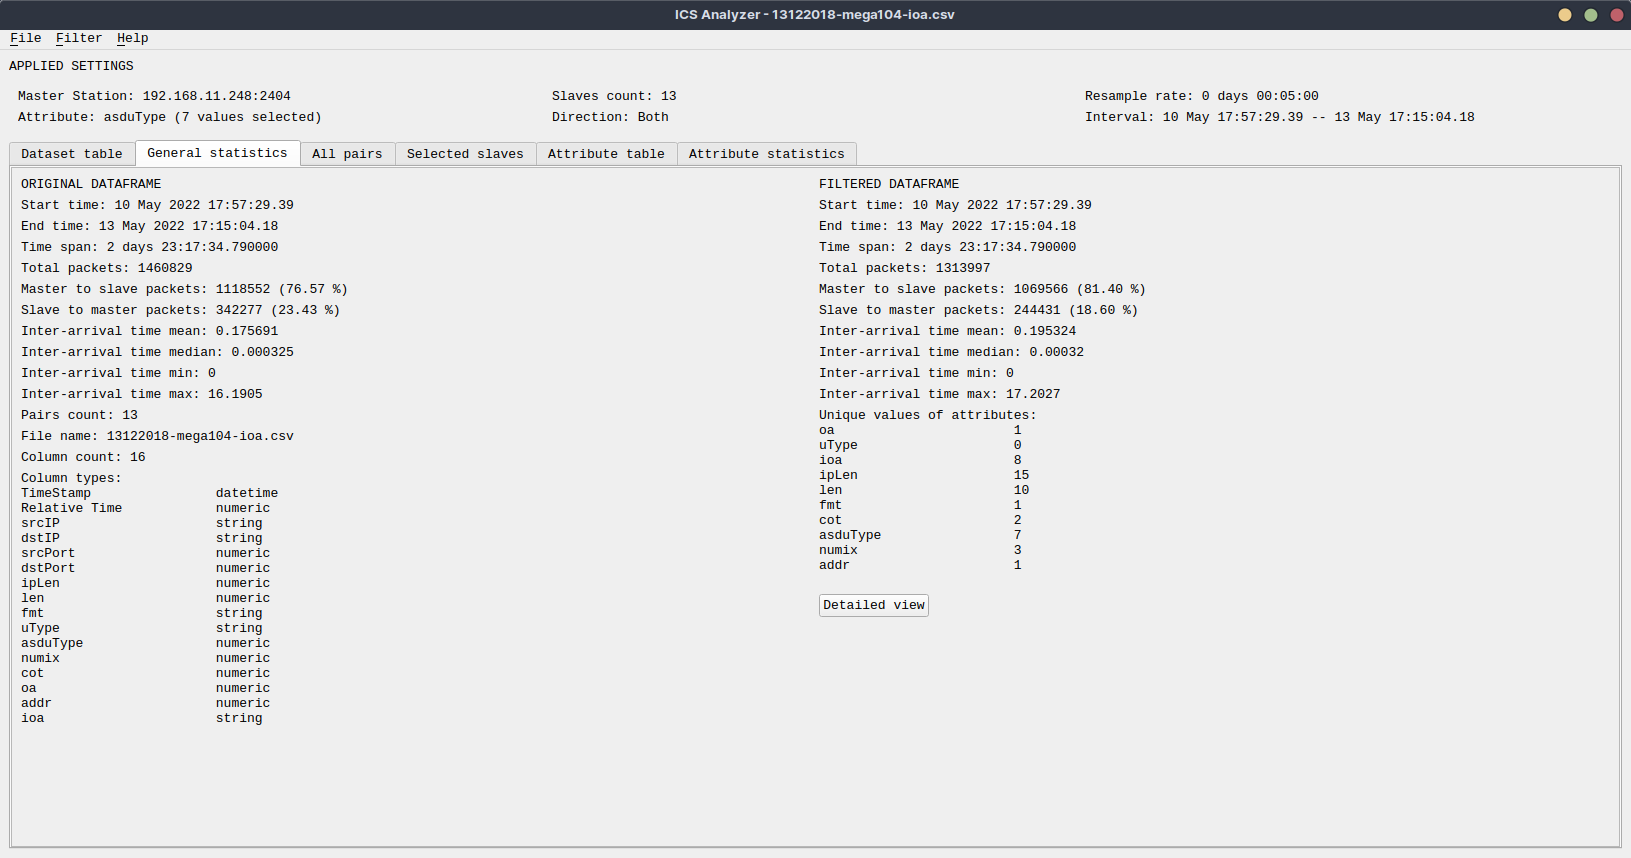
\includegraphics[width=1\textwidth]{obrazky-figures/tabs/tab2.png}
	\caption{General statistics}
	\label{fig:tab2}
    \end{figure}
    
    
    \begin{figure}[H]
    	\centering
    	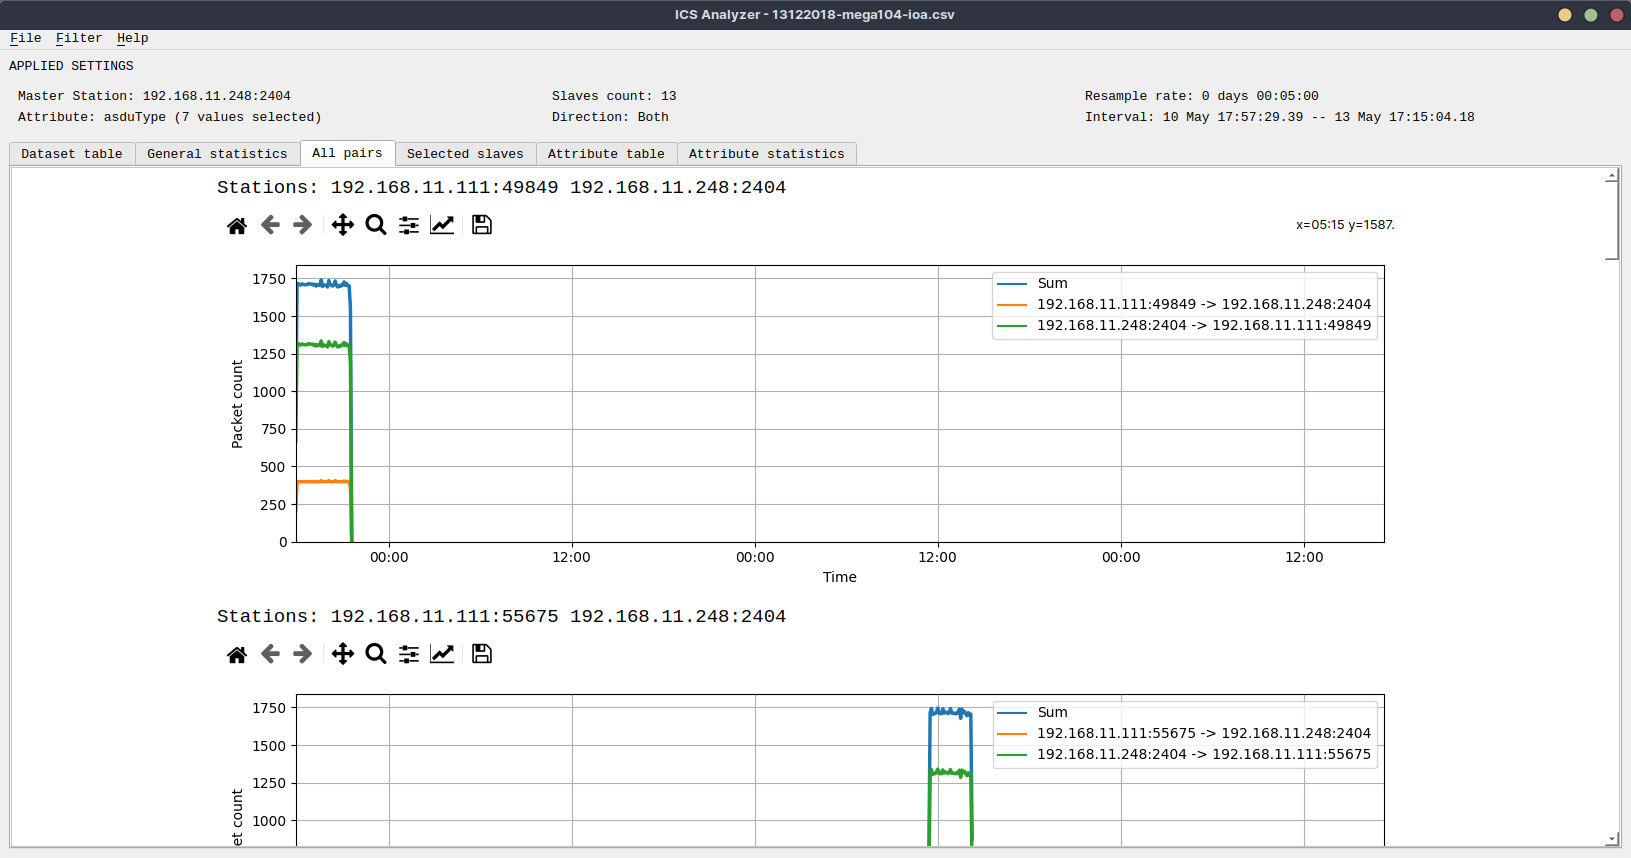
\includegraphics[width=1\textwidth]{obrazky-figures/tabs/tab3.png}
    	\caption{All pairs}
    	\label{fig:tab3}
    \end{figure}
    
    
    \begin{figure}[H]
    	\centering
    	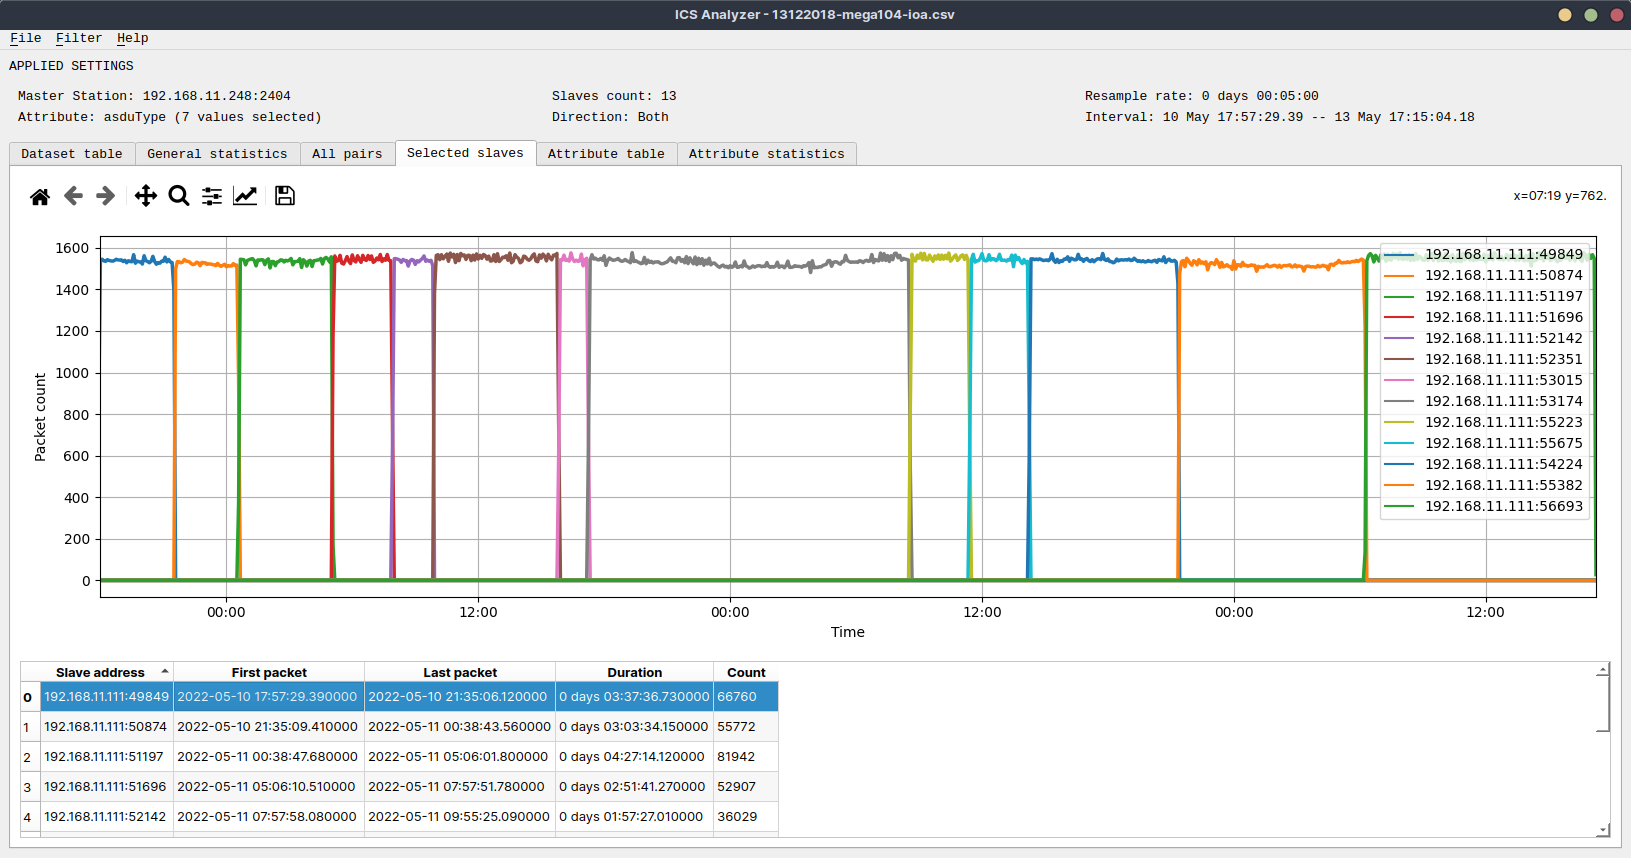
\includegraphics[width=1\textwidth]{obrazky-figures/tabs/tab4.png}
    	\caption{Selected slaves}
    	\label{fig:tab4}
    \end{figure}
    
    \begin{figure}[H]
    	\centering
    	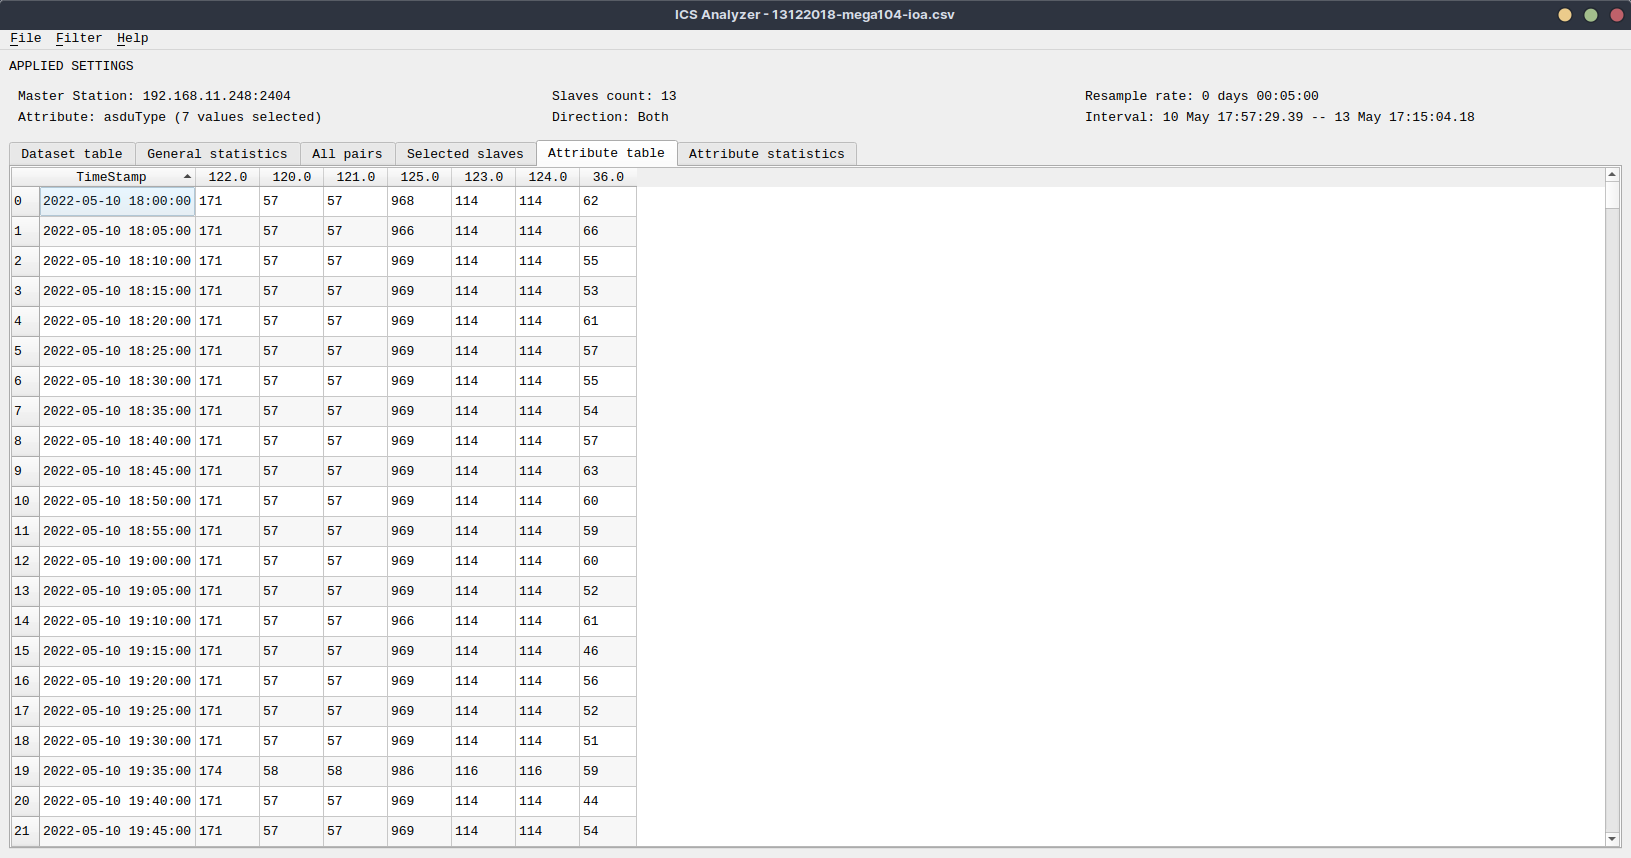
\includegraphics[width=1\textwidth]{obrazky-figures/tabs/tab5.png}
    	\caption{Attribute table}
    	\label{fig:tab5}
    \end{figure}
    
    
    \begin{figure}[H]
    	\centering
    	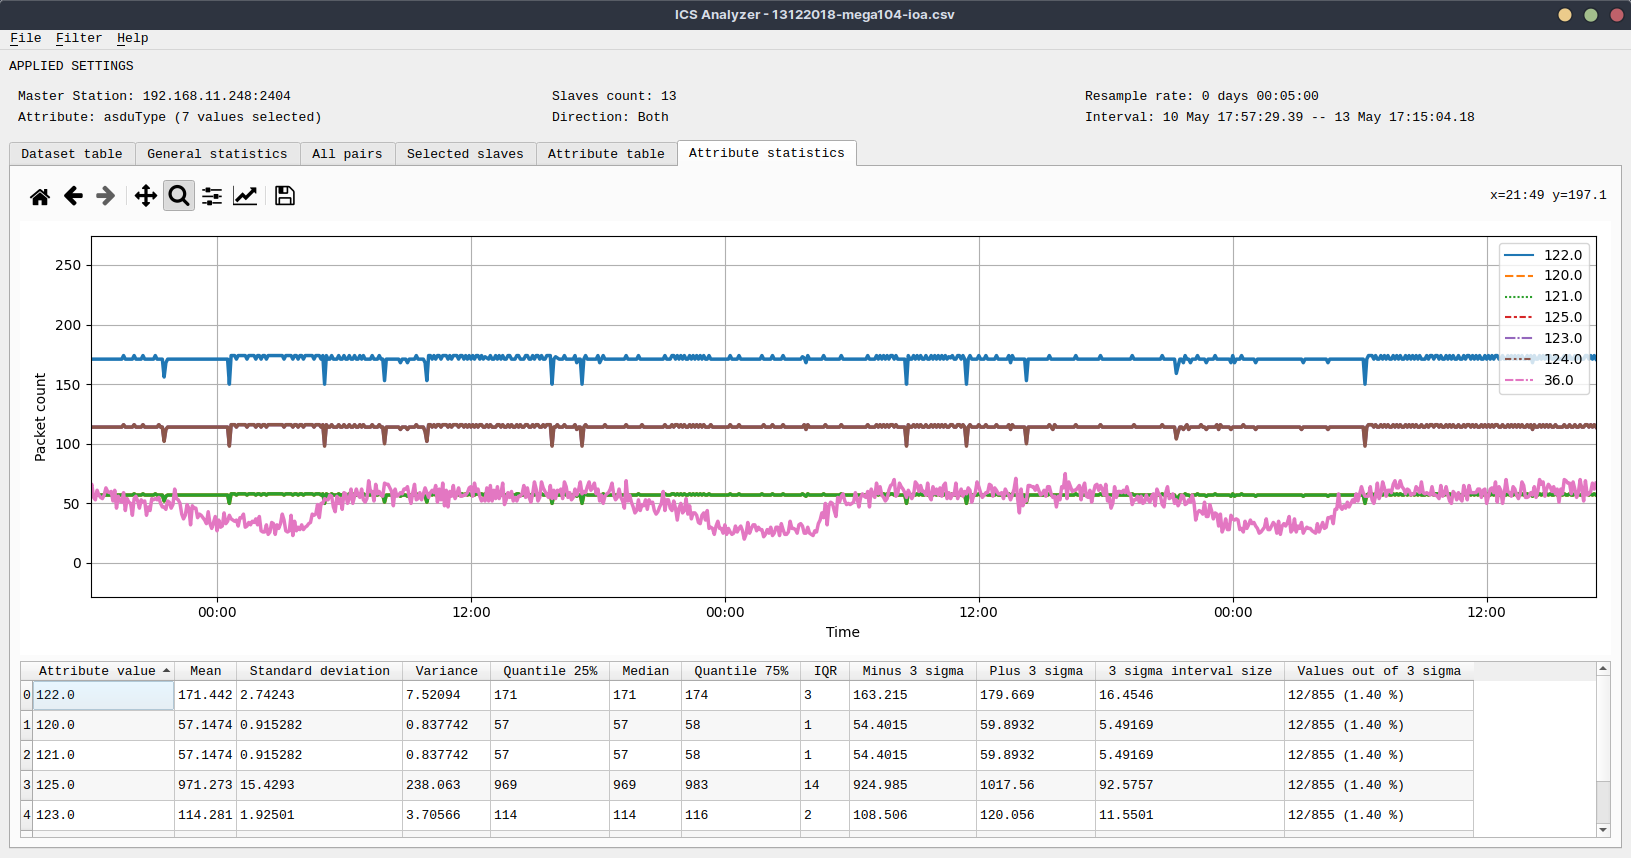
\includegraphics[width=1\textwidth]{obrazky-figures/tabs/tab6.png}
    	\caption{Attribute statistics}
    	\label{fig:tab6}
    \end{figure}



% \chapter{Stromová struktura zdrojového kódu}
    
% \begin{figure}[H]
%     \centering
%     \begin{forest}
%       for tree={
%         font=\ttfamily,
%         grow'=0,
%         child anchor=west,
%         parent anchor=south,
%         anchor=west,
%         calign=first,
%         edge path={
%           \noexpand\path [draw, \forestoption{edge}]
%           (!u.south west) +(7.5pt,0) |- node[fill,inner sep=1.25pt] {} (.child anchor)\forestoption{edge label};
%         },
%         before typesetting nodes={
%           if n=1
%             {insert before={[,phantom]}}
%             {}
%         },
%         fit=band,
%         before computing xy={l=15pt},
%       }
%     [src
%       [dsmanipulator
%         [\_\_init\_\_.py]
%         [dataobjects.py]
%         [dsanalyzer.py]
%         [dscreator.py]
%         [dsloader.py]
%       ]
%       [app
%         [\_\_init\_\_.py]
%         [datamodels.py]
%         [dialogs.py]
%         [eventhandler.py]
%         [opencsvwizard.py]
%         [qtwaitingspinner.py]
%         [tabs.py]
%         [widgets.py]
%         [windows.py]
%         [workers.py]
%       ]
%       [main.py]
%     ]
%     \end{forest}
% 	\caption{Stromová struktura souborů se zdrojovým kódem.}
% 	\label{tree_struct}
% \end{figure}


